\documentclass[11pt,a4paper]{article}
\usepackage[utf8]{inputenc}
\usepackage[T1]{fontenc}
\usepackage[spanish,es-nodecimaldot,es-tabla]{babel}
\usepackage{lmodern}
\usepackage{amsmath,amssymb}
\usepackage{graphicx}
\usepackage{booktabs,longtable,array,tabularx,multirow}
\usepackage{ragged2e}
\usepackage{siunitx}
\usepackage{enumitem}
\usepackage{geometry}
\usepackage{float}
\usepackage{xcolor}
\usepackage{pdflscape}
\usepackage{caption,subcaption}
\usepackage{fancyhdr}
\usepackage[hidelinks]{hyperref}
\hypersetup{colorlinks=true,linkcolor=black,citecolor=black,urlcolor=blue,
  pdftitle={Micro-ohmímetro de precisión v2},pdfauthor={E. A. Pacheco J.; J. T. Albarracín C.}}
\geometry{top=22mm,bottom=22mm,left=20mm,right=20mm}
\graphicspath{{figuras/}}
\sisetup{output-decimal-marker={,},per-mode=symbol,group-separator={.}}
\renewcommand{\arraystretch}{1.2}
\setlength{\parindent}{0pt}
\setlength{\parskip}{0.45em}
\setlength{\headheight}{14pt}
\pagestyle{fancy}\fancyhf{}
\lhead{Micro-ohmímetro de precisión -- versión 2}\rhead{UIS -- E3T}\cfoot{\thepage}
\newcolumntype{Y}{>{\RaggedRight\arraybackslash}X}
\newcommand{\repo}{https://github.com/EDWARDPJ26/microohmetro-uis}
\newcommand{\repof}[1]{\href{\repo/blob/v1.0/#1}{\texttt{\detokenize{#1}}}}
\newcommand{\fuente}[1]{\\[-1mm]{\footnotesize\textit{Fuente: #1}}}
\newcommand{\PENDIENTE}[1]{\textcolor{red}{\textbf{[PENDIENTE: #1]}}}

\begin{document}
% =====================================================================================
\begin{titlepage}
\centering
\vspace*{8mm}
{\Large\textbf{UNIVERSIDAD INDUSTRIAL DE SANTANDER}}\\[2mm]
{\large Escuela de Ingenierías Eléctrica, Electrónica y de Telecomunicaciones}\\[14mm]
{\LARGE\textbf{DISEÑO DE UN MICRO-OHMÍMETRO DE PRECISIÓN}}\\[3mm]
{\Large \SI{1}{m\ohm} -- \SI{1}{\ohm}, portátil, con medición Kelvin de 4 hilos}\\[3mm]
{\large Informe final consolidado -- versión 2 (con las correcciones del docente)}\\[16mm]
\textbf{Edward Andrés Pacheco Jurado} -- 2222236 -- A1A\\[2mm]
\textbf{Joseph Thomas Albarracín Contreras} -- 2220415 -- A1B\\[14mm]
Diseño de Sistemas Electrónicos\\ Docente: Jaime Barrero\\[18mm]
Bucaramanga, Santander -- 2026\\[10mm]
\begin{minipage}{0.86\textwidth}\small
Repositorio de respaldo (esquemáticos, PCB, Gerbers, simulaciones, datos, firmware, imágenes en alta resolución y datasheets):
\href{\repo}{\texttt{github.com/EDWARDPJ26/microohmetro-uis}} (versión etiquetada \texttt{v1.0}).
\end{minipage}
\end{titlepage}

\pagenumbering{roman}
\tableofcontents\clearpage
\listoffigures\listoftables\clearpage
\pagenumbering{arabic}

% =====================================================================================
\section*{Resumen}
\addcontentsline{toc}{section}{Resumen}
Se presenta el diseño completo de un micro-ohmímetro portátil para el rango \SI{1}{m\ohm}--\SI{1}{\ohm}. La versión 2 incorpora todas las correcciones del docente: corriente de prueba \textbf{pulsada de \SI{1,04}{A}}, referencia de tensión integrada (sin divisores), medición \textbf{Kelvin con bornes banana de \SI{4}{mm}}, uso del \textbf{PGA, buffers y filtros del AD7124-4}, medición \textbf{ratiométrica de dos niveles} que cancela offsets y FEM termoeléctricas, cargador conmutado rápido con \textbf{USB-C Power Delivery}, protección contra polaridad inversa, microcontrolador actualizado \textbf{ESP32-C3 con USB nativo y OTA}, batería LiPo integrada en la PCB y análisis de \textbf{Montecarlo y peor caso}. Las simulaciones en PSpice con los modelos oficiales de TI muestran un error sistemático de \SI{-0,0054}{\percent} (calibrable), inmunidad total a una FEM de \SI{\pm10}{\micro V} y una dispersión por tolerancias igual a la del shunt: $\sigma=\SI{0,057}{\percent}$ con un shunt del \SI{0,1}{\percent}. El diseño anterior, con amplificador diferencial discreto, presentaba $\sigma=\SI{88}{\percent}$ en \SI{10}{m\ohm}.

% =====================================================================================
\section{Requerimientos y correcciones atendidas}
\begin{table}[H]\centering\small
\caption{Correcciones del docente y cómo se atendieron.}\label{tab:correcciones}
\begin{tabularx}{\textwidth}{>{\RaggedRight}p{5.2cm}Y}
\toprule
\textbf{Corrección} & \textbf{Solución en la versión 2}\\\midrule
Protección de polaridad de la batería & 2$\times$AO3401A en paralelo (P-MOS, $\approx$\SI{43}{m\ohm}), sección~\ref{sec:energia}.\\
Bornes banana Kelvin y conector de batería seguro & 4 bornes de \SI{4}{mm} (I+, S+, S$-$, I$-$); JST XH SMD de 3 pines con NTC.\\
Vref estable sin divisores & REF3325 (\SI{2,5}{V}, \SI{0,15}{\percent}, \SI{30}{ppm/\celsius}).\\
Corriente de 1--2 A, pulsada & \SI{1,042}{A} / \SI{0,502}{A}, pulsos de \SI{120}{ms} cada \SI{1}{s}.\\
Offset del OPA391 & OPA388 zero-drift + medición ratiométrica de 2 niveles; simulado con $\pm V_{OS}$.\\
USB único para carga y programación & USB-C: VBUS al cargador, D+/D$-$ al USB nativo del ESP32-C3.\\
ESP32 NRND & ESP32-C3-WROOM-02 (RISC-V, BLE 5, USB-Serial/JTAG).\\
Carga más rápida & BQ25895 conmutado, \SI{2}{A} (1C), $\approx$\SI{1,5}{h}.\\
USB-C PD 240 W y materiales & STUSB4500 (sink, 9 V/2 A, compatible con cargadores EPR); tabla~\ref{tab:materiales}.\\
OTA, PGA y filtros del ADC & Particiones OTA dobles; PGA 128/16/2, buffers y post-filtro de 25 SPS.\\
Montecarlo de tolerancias & 300 corridas + Worst-Case en PSpice, sección~\ref{sec:sim}.\\
Footprints y 3D; batería en la PCB; placa compacta & Footprints oficiales de KiCad 10; LiPo en la cara inferior, sección~\ref{sec:pcb}.\\
Informe único, imágenes y GitHub & Este documento; figuras vectoriales; repositorio enlazado.\\
\bottomrule\end{tabularx}
\end{table}

\begin{table}[H]\centering\small
\caption{Especificaciones del instrumento.}\label{tab:spec}
\begin{tabular}{ll}\toprule
Rango & \SI{1}{m\ohm} -- \SI{1}{\ohm} (3 rangos automáticos del PGA)\\
Corriente de prueba & \SI{1,042}{A} y \SI{0,502}{A}, pulsada (\SI{120}{ms} / \SI{1}{s})\\
Resolución (1 m$\Omega$, una lectura) & $\approx$\SI{0,011}{\percent} (ruido \SI{0,063}{\micro V} rms, G = 128)\\
Error por tolerancias (sin calibrar) & $\pm$\SI{0,1}{\percent} con shunt de \SI{0,1}{\percent}\\
Alimentación & LiPo 1S \SI{2000}{mAh}; USB-C PD (5/9 V)\\
Autonomía (estimada) & $\approx$\SI{10}{h} midiendo; $\approx$\SI{40}{h} en reposo\\
Comunicación & BLE 5 (aplicación Android) y USB\\
PCB & 4 capas, 64\,mm $\times$ 116\,mm, batería en la cara inferior\\\bottomrule
\end{tabular}\end{table}

% =====================================================================================
\section{Arquitectura general}
La figura~\ref{fig:bloques} es la hoja raíz del esquemático jerárquico (KiCad 10). Cada bloque es una hoja de detalle (anexo~\ref{anx:sch}). La medición se basa en:
\begin{equation}
R_{DUT}=R_S\,\frac{V_{DUT,H}-V_{DUT,L}}{V_{RS,H}-V_{RS,L}}
\label{eq:ratiometrica}\end{equation}
donde $H$ y $L$ son los dos niveles de corriente y $V_{RS}$ es la caída en el shunt $R_S=\SI{0,12}{\ohm}$. La ecuación~\eqref{eq:ratiometrica} no depende del valor exacto de la corriente, de la referencia ni de la ganancia del INA181, y la diferencia entre niveles cancela offsets del ADC y FEM termoeléctricas de los contactos.

\begin{figure}[H]\centering
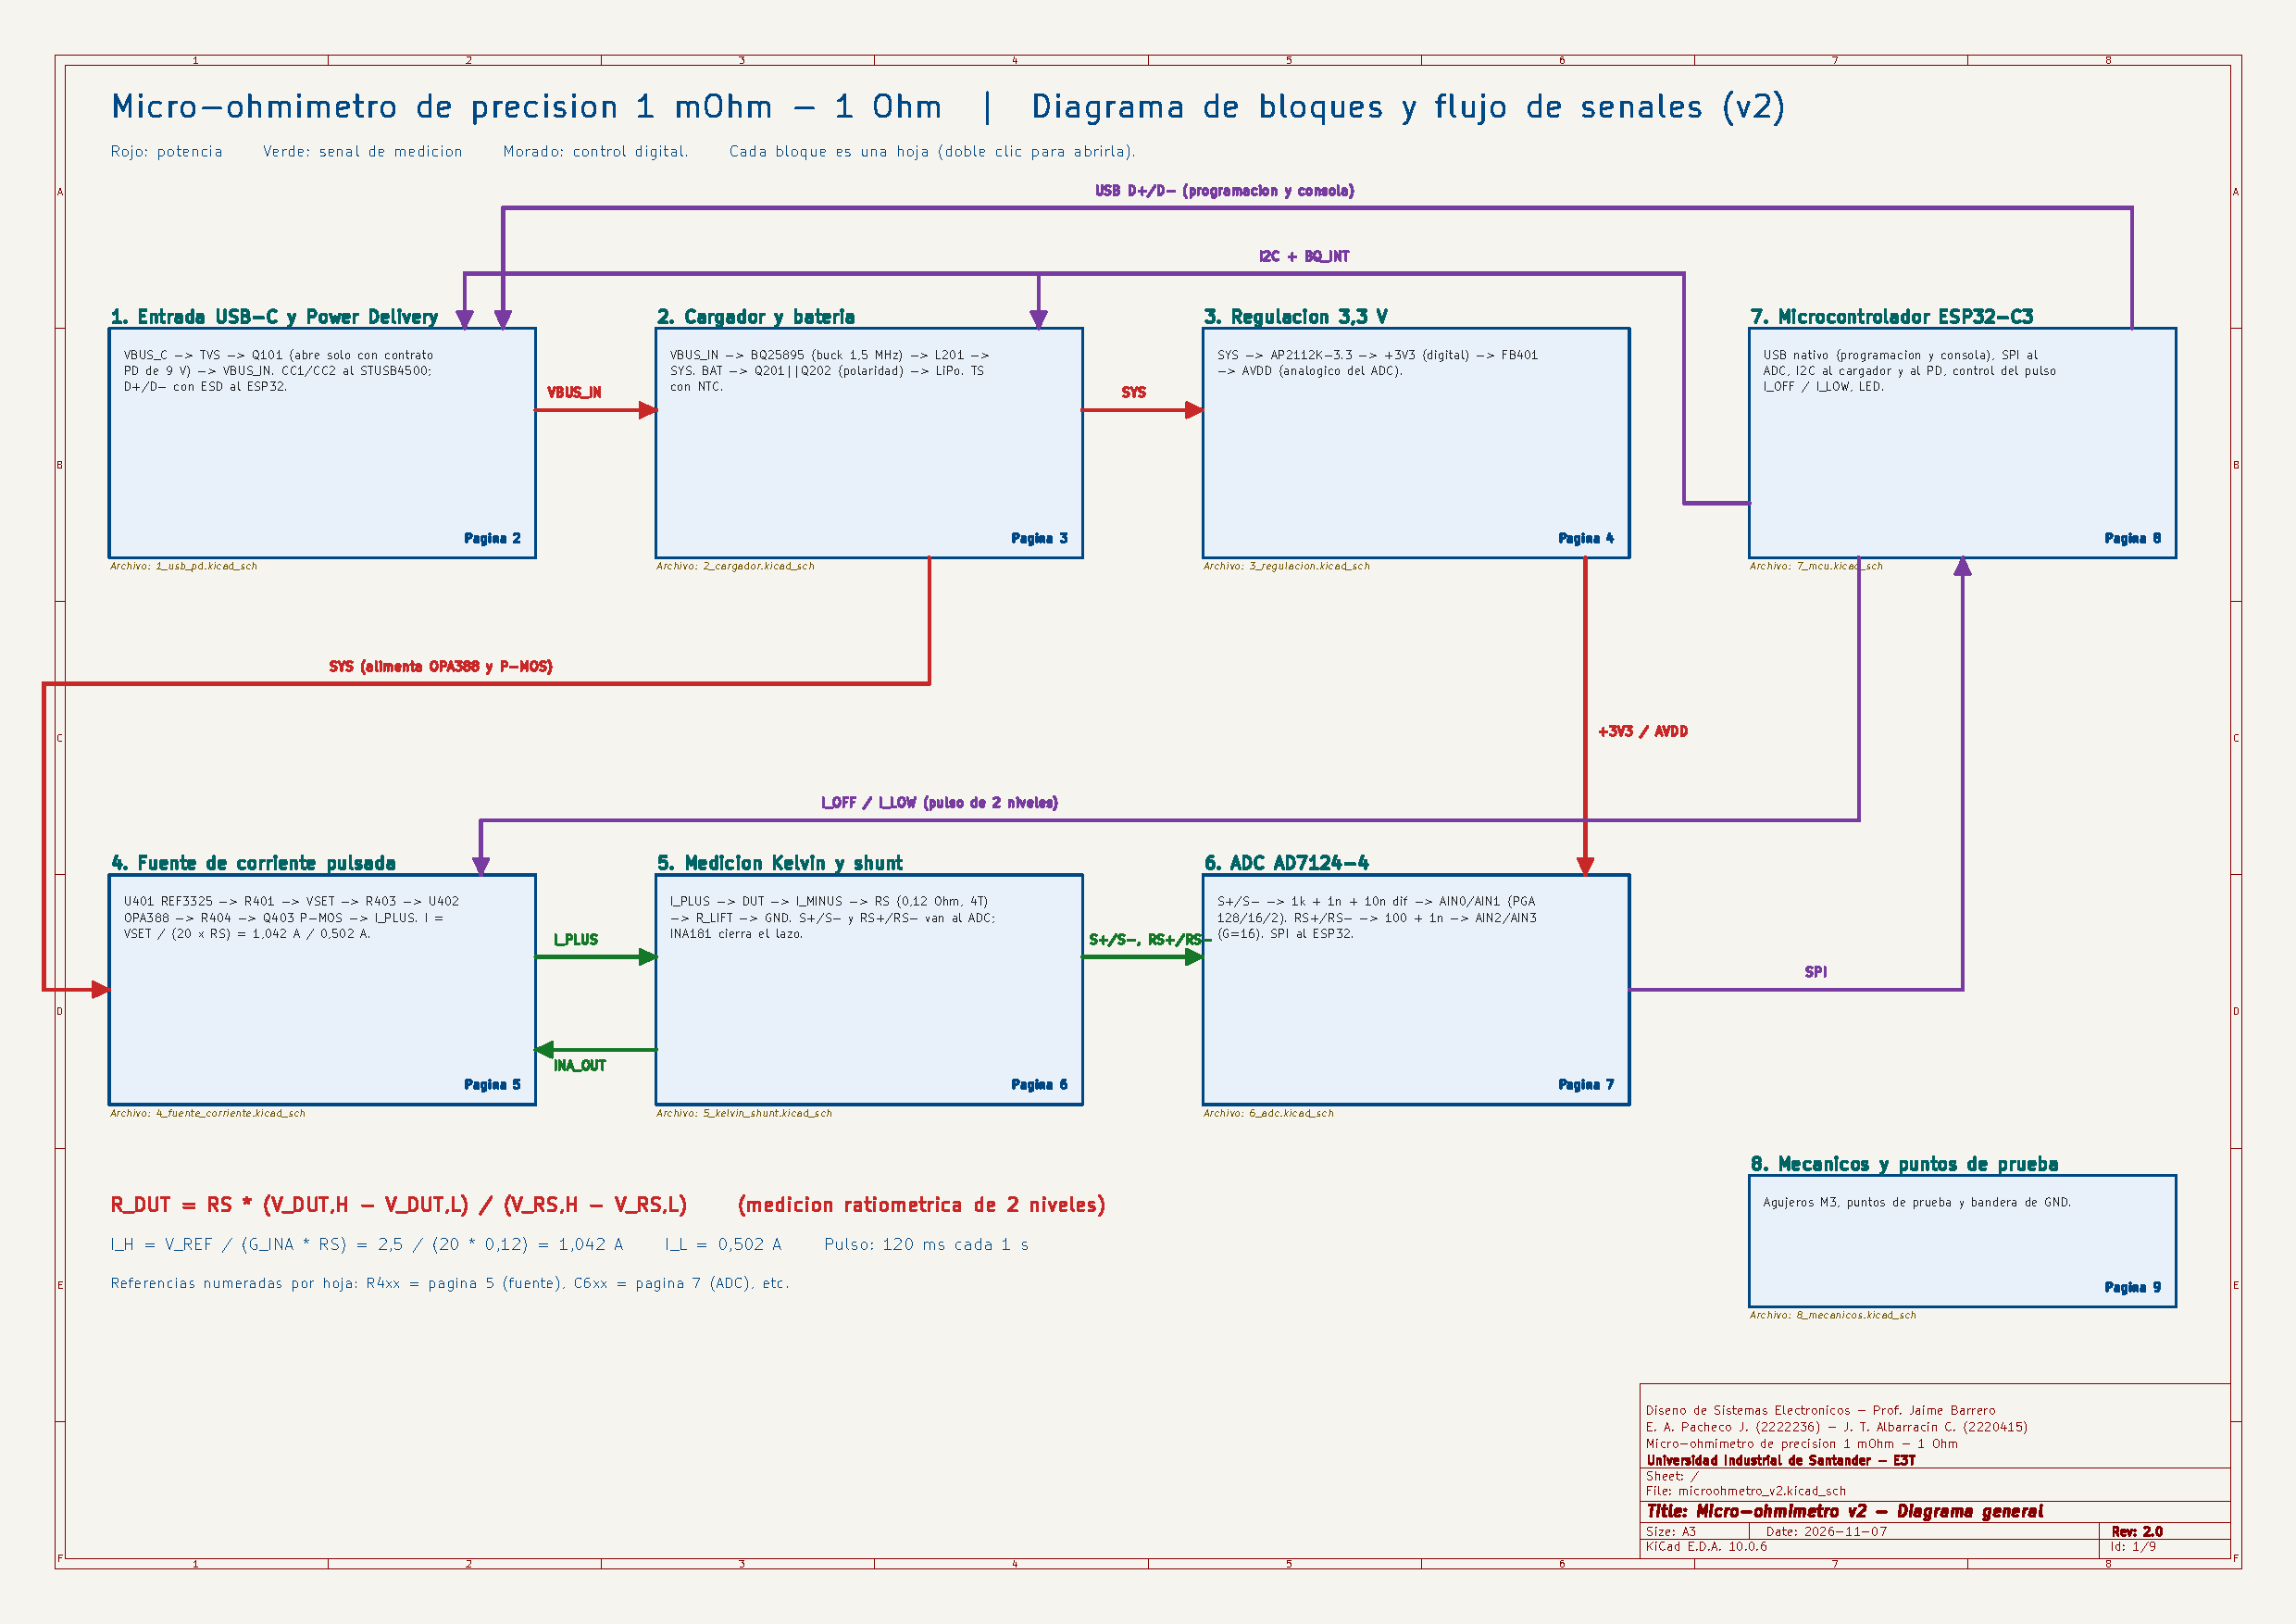
\includegraphics[page=1,width=\textwidth]{esquematico_v2.pdf}
\caption{Esquemático, hoja raíz: diagrama de bloques y flujo de señales (rojo: potencia, verde: medición, morado: control).}\label{fig:bloques}
\fuente{elaboración propia en KiCad 10; archivo \repof{hardware/kicad/microohmetro_v2.kicad_sch}.}
\end{figure}

% =====================================================================================
\section{Fuente de corriente pulsada de dos niveles}
La REF3325 fija $V_{SET}$ a través de R401 (\SI{10}{k\ohm}) y C402 (\SI{22}{nF}, arranque suave). El OPA388 compara $V_{SET}$ con la salida del INA181A1 ($G=\SI{20}{V/V}$) y controla el P-MOS NTD25P03L (DPAK):
\begin{equation}
I=\frac{V_{SET}}{G_{INA}\,R_S}=\frac{\SI{2,5}{V}}{20\cdot\SI{0,12}{\ohm}}=\SI{1,042}{A},\qquad I_L=\frac{\SI{1,205}{V}}{2,4}=\SI{0,502}{A}.
\end{equation}
Q402 conecta \SI{9,31}{k\ohm} para el nivel bajo y Q401 anula $V_{SET}$ (corriente apagada por defecto al arrancar). La referencia sigue siendo la REF3325; el valor exacto de $I_L$ no influye porque $V_{RS}$ se mide en ambos niveles. La disipación pico del P-MOS es \SI{3,5}{W}, con \SI{0,43}{W} de promedio al \SI{12}{\percent} de ciclo útil ($\approx$\SI{+22}{\celsius}). El margen de tensión en el peor caso (\SI{1}{\ohm}, batería en \SI{3,5}{V}) es \SI{1,52}{V}.

\begin{figure}[H]\centering
\includegraphics[page=5,width=\textwidth,trim=10mm 40mm 10mm 25mm,clip]{esquematico_v2.pdf}
\caption{Hoja 4: fuente de corriente pulsada (cadena cableada pin a pin).}\label{fig:fuente}
\end{figure}

% =====================================================================================
\section{Medición Kelvin y adquisición con el AD7124-4}
I+ e I$-$ conducen la corriente; S+ y S$-$ solo miden tensión. El shunt de 4 terminales (WSK2512) entrega $V_{RS}$ al INA181 y al ADC. $R_{LIFT}=\SI{0,68}{\ohm}$ eleva el modo común por encima del mínimo del PGA ($V_{CM}\geq \SI{0,1}{V}+\SI{0,5}{V}/G$; nota 8 del datasheet). Las entradas llevan \SI{1}{k\ohm} + \SI{1}{nF} C0G por línea, \SI{10}{nF} C0G diferencial y clamp BAT54S.

\begin{table}[H]\centering\small
\caption{Configuración de canales del AD7124-4 (referencia interna de 2,5 V, post-filtro de 25 SPS).}\label{tab:adc}
\begin{tabular}{lllll}\toprule
Canal & Entradas & PGA & Rango & Uso\\\midrule
CH0 & AIN0/AIN1 (S+/S$-$) & 128 & $\pm$\SI{19,5}{mV} & $R\leq\SI{15}{m\ohm}$\\
CH1 & AIN0/AIN1 & 16 & $\pm$\SI{156}{mV} & $R\leq\SI{120}{m\ohm}$\\
CH2 & AIN0/AIN1 & 2 & $\pm$\SI{1,25}{V} & $R\leq\SI{1}{\ohm}$\\
CH3 & AIN2/AIN3 (RS) & 16 & $\pm$\SI{156}{mV} & $V_{RS}=60/125$ mV\\\bottomrule
\end{tabular}\end{table}

\begin{figure}[H]\centering
\begin{subfigure}{0.49\textwidth}\includegraphics[page=6,width=\textwidth,trim=10mm 40mm 20mm 25mm,clip]{esquematico_v2.pdf}\caption{Hoja 5: bornes Kelvin, shunt e INA181.}\end{subfigure}
\begin{subfigure}{0.49\textwidth}\includegraphics[page=7,width=\textwidth,trim=10mm 40mm 10mm 25mm,clip]{esquematico_v2.pdf}\caption{Hoja 6: AD7124-4 con filtros y protección.}\end{subfigure}
\caption{Cadena de medición.}\label{fig:medicion}\end{figure}

\textbf{Secuencia por medición} ($\approx$\SI{240}{ms}): nivel $I_L$ (5 ms de asentamiento + conversión de $V_{DUT}$ y $V_{RS}$), nivel $I_H$ (igual), corriente apagada. El firmware elige automáticamente el PGA y aplica la ecuación~\eqref{eq:ratiometrica}.

% =====================================================================================
\section{Energía: USB-C PD, cargador, polaridad y regulación}\label{sec:energia}
\begin{itemize}[nosep]
\item \textbf{USB-C + STUSB4500}: negocia 9 V/2 A (PDO2) o 5 V/3 A; Q101 conecta VBUS solo con un contrato válido; TVS SMBJ12A. Compatible con cargadores de \SI{240}{W} (EPR), que también ofrecen los perfiles estándar.
\item \textbf{BQ25895} (buck de 1,5 MHz): $I_{CHG}=\SI{2048}{mA}$ por I\textsuperscript{2}C, $I_{IN,max}=355/R_{ILIM}=\SI{2,0}{A}$, temporizador desactivado, NTC en TS ($R_{T1}=\SI{5,23}{k\ohm}$, $R_{T2}=\SI{30,1}{k\ohm}$). Carga completa en $\approx$\SI{1,5}{h}.
\item \textbf{Polaridad inversa}: 2$\times$AO3401A en paralelo entre el conector y BAT.
\item \textbf{AP2112K-3.3} desde SYS; AVDD del ADC filtrado con ferrita.
\end{itemize}

\begin{table}[H]\centering\small
\caption{Presupuesto energético sobre SYS.}\label{tab:energia}
\begin{tabular}{lrl}\toprule
Bloque & Corriente media & Base\\\midrule
Pulso de \SI{1,042}{A} al \SI{12}{\percent} & \SI{125}{mA} & Diseño\\
ESP32-C3 con BLE & 30--45 mA & Estimado (a medir)\\
AD7124-4 + OPA388 + INA181 + REF & $\approx$\SI{3}{mA} & Datasheets\\
\textbf{Total midiendo} & \textbf{$\approx$160--175 mA} & \textbf{$\approx$10 h} con \SI{2000}{mAh}\\\bottomrule
\end{tabular}\end{table}

% =====================================================================================
\section{Microcontrolador y firmware}
ESP32-C3-WROOM-02-N4: USB nativo (programación y consola sin conversor), SPI al ADC (GPIO5/6/7/10), I\textsuperscript{2}C al BQ25895 y al STUSB4500 (GPIO4/8), control del pulso (I\_OFF en GPIO0, I\_LOW en GPIO3), LED, RESET y BOOT. Firmware: máquina de estados de medición de dos niveles, rango automático del PGA, calibración interna del ADC por ganancia más calibración de sistema con una resistencia patrón, BLE hacia la aplicación y \textbf{OTA} (dos particiones de app, \emph{rollback} si el ADC no responde).

% =====================================================================================
\section{Simulaciones (PSpice 22.1)}\label{sec:sim}
Se usaron los modelos oficiales de TI del OPA388 (OPA4388) y del INA181A1. Los cables de fuerza se simularon con \SI{20}{m\ohm} y los de sensado con \SI{100}{m\ohm}. Archivos: \repof{simulaciones/}.

\begin{table}[H]\centering\small
\caption{Resultados DC (S1): idénticos con SYS = 3,5 V y 4,35 V.}\label{tab:s1}
\begin{tabular}{lcccc}\toprule
$R_{DUT}$ & $I_L$ (A) & $I_H$ (A) & $R$ medida & Error\\\midrule
\SI{1}{m\ohm} & 0,50233 & 1,04181 & \SI{0,99995}{m\ohm} & \SI{-0,0054}{\percent}\\
\SI{10}{m\ohm} & 0,50233 & 1,04181 & \SI{9,9995}{m\ohm} & \SI{-0,0054}{\percent}\\
\SI{100}{m\ohm} & 0,50233 & 1,04181 & \SI{99,995}{m\ohm} & \SI{-0,0054}{\percent}\\
\SI{1}{\ohm} & 0,50233 & 1,04181 & \SI{0,99995}{\ohm} & \SI{-0,0054}{\percent}\\\bottomrule
\end{tabular}\end{table}

\begin{figure}[H]\centering
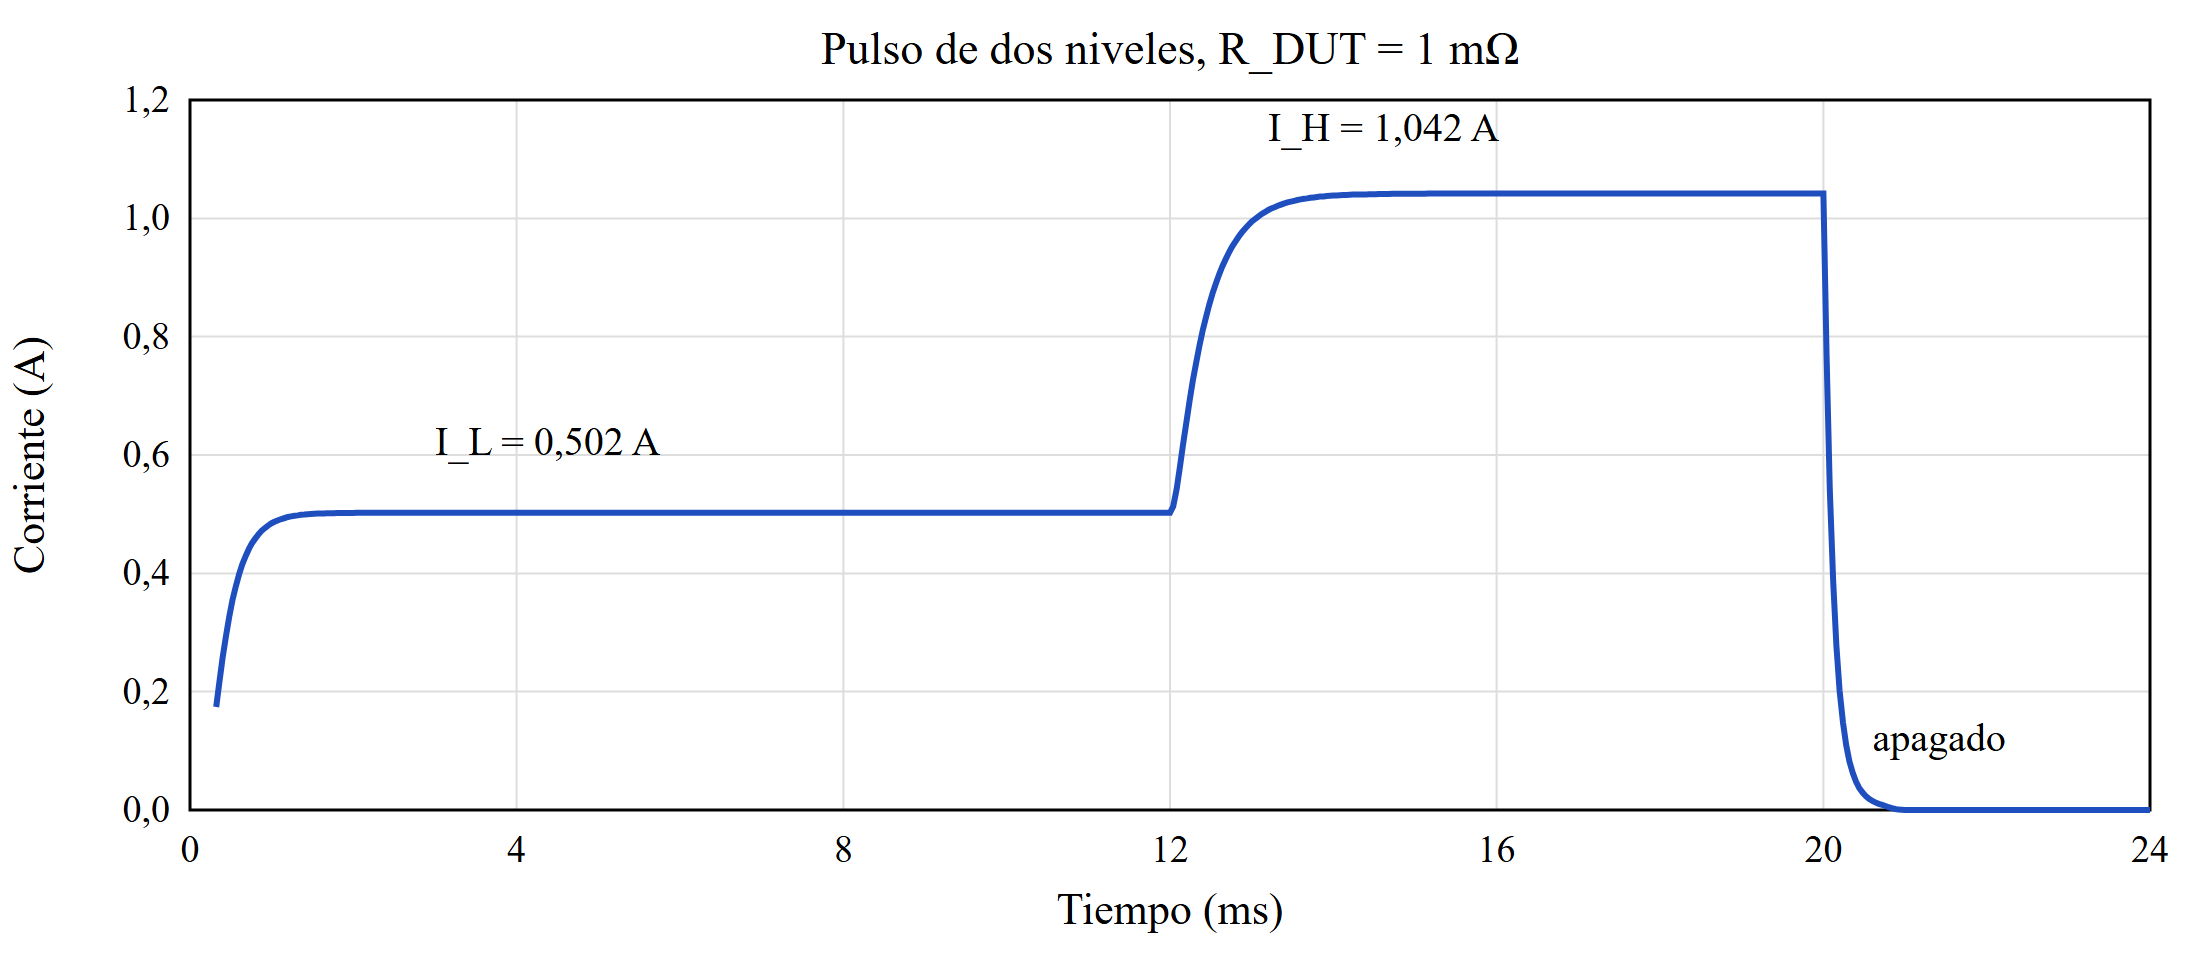
\includegraphics[width=0.92\textwidth]{graf_pulso.png}
\caption{S2: pulso de dos niveles ($I_L\to I_H$ a 12 ms, apagado a 20 ms). Sin sobrepico; asentamiento de 3,3 ms al 0,01 \%.}\label{fig:pulso}
\end{figure}

\begin{table}[H]\centering\small
\caption{S3: efecto del offset del OPA388 y de la FEM termoeléctrica ($R_{DUT}=\SI{1}{m\ohm}$).}\label{tab:s3}
\begin{tabular}{cccc}\toprule
$V_{OS}$ OPA388 & FEM en S+ & Error con 2 niveles & Error con 1 nivel\\\midrule
$\pm$\SI{5}{\micro V} & \SI{-10}{\micro V} & \SI{-0,0054}{\percent} & \SI{+0,954}{\percent}\\
$\pm$\SI{5}{\micro V} & 0 & \SI{-0,0054}{\percent} & \SI{-0,005}{\percent}\\
$\pm$\SI{5}{\micro V} & \SI{+10}{\micro V} & \SI{-0,0054}{\percent} & \SI{-0,965}{\percent}\\\bottomrule
\end{tabular}\end{table}

\begin{figure}[H]\centering
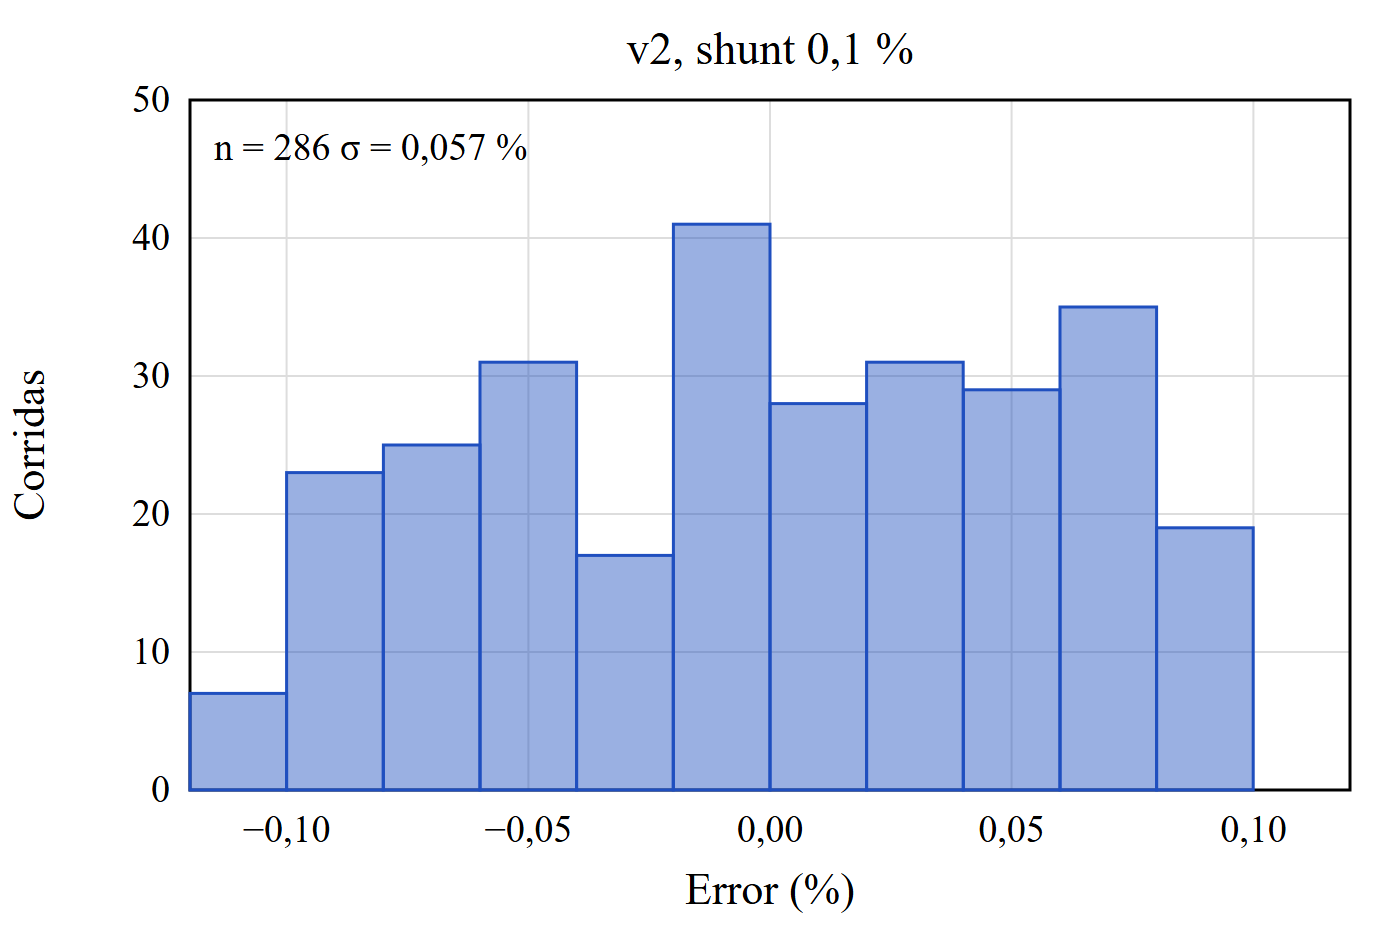
\includegraphics[width=0.49\textwidth]{graf_mc_v2.png}\hfill
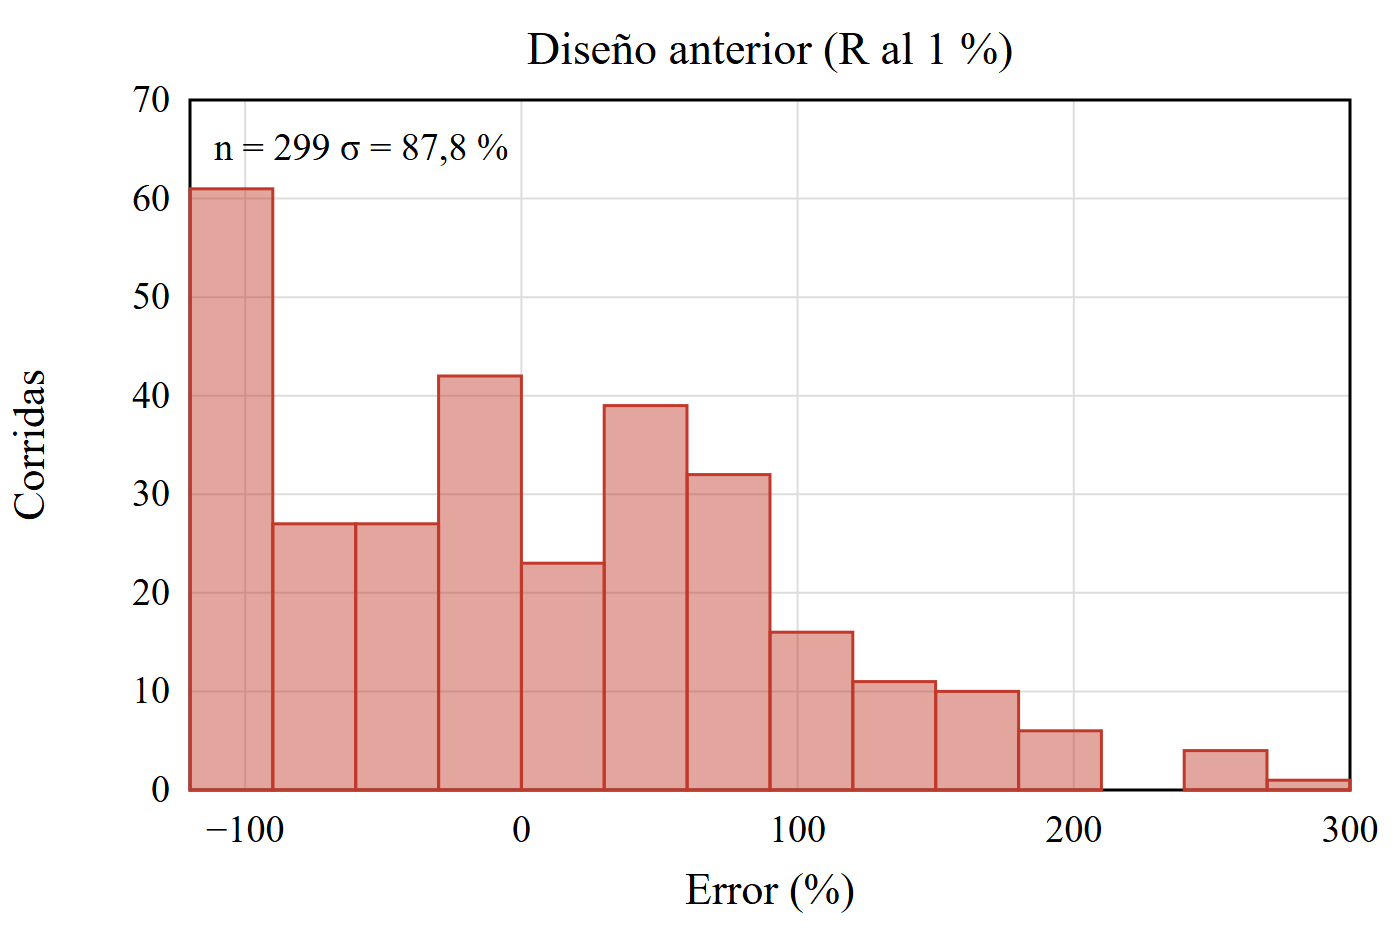
\includegraphics[width=0.49\textwidth]{graf_mc_anterior.png}
\caption{S4: Montecarlo (300 corridas). Izquierda: $\sigma=\SI{0,057}{\percent}$. Derecha: $\sigma=\SI{88}{\percent}$ en \SI{10}{m\ohm}.}\label{fig:mc}
\end{figure}

\begin{table}[H]\centering\small
\caption{S4/S5: Montecarlo y sensibilidad (Worst-Case).}\label{tab:mc}
\begin{tabular}{lccc}\toprule
Caso & Media & $\sigma$ & Rango\\\midrule
v2, $R_S$ 1 \%, \SI{1}{m\ohm} & \SI{+0,025}{\percent} & \SI{0,57}{\percent} & $\pm$\SI{0,99}{\percent}\\
v2, $R_S$ 1 \%, \SI{1}{\ohm} & \SI{+0,022}{\percent} & \SI{0,56}{\percent} & $\pm$\SI{0,99}{\percent}\\
v2, $R_S$ \textbf{0,1 \%}, \SI{1}{m\ohm} & \SI{-0,001}{\percent} & \textbf{\SI{0,057}{\percent}} & $\pm$\SI{0,11}{\percent}\\
Diseño anterior, \SI{10}{m\ohm} & \SI{+5,7}{\percent} & \SI{88}{\percent} & $-100$ \ldots $+284$ \%\\\midrule
\multicolumn{4}{l}{Sensibilidad: $R_S$ $-0,99$ \%/\%; R\_FP $+0,047$; R\_FN $-0,035$; resto $\leq0,012$. Peor caso total: $+1,02$ \%.}\\\bottomrule
\end{tabular}\end{table}

% =====================================================================================
\section{Presupuesto de error}
\begin{table}[H]\centering\small
\caption{Presupuesto de error estimado ($R_{DUT}=\SI{1}{m\ohm}$, una medición).}\label{tab:error}
\begin{tabular}{lcl}\toprule
Fuente & Contribución & Tratamiento\\\midrule
Tolerancia de $R_S$ (0,1 \%) & \SI{0,10}{\percent} & Calibración con patrón $\to$ \SI{0,01}{\percent}\\
TCR de $R_S$ (50 ppm/°C, $\Delta T=\SI{10}{\celsius}$) & \SI{0,05}{\percent} & Pulsado (bajo autocalentamiento)\\
Ruido del ADC (G = 128) & \SI{0,011}{\percent} & Promedio $\times$16 $\to$ \SI{0,003}{\percent}\\
Bias del INA181 (sistemático) & \SI{0,0054}{\percent} & Calibración\\
Offset ADC/OPA y FEM & $\approx$0 & Cancelado (2 niveles)\\\midrule
\textbf{RSS sin calibrar / calibrado} & \textbf{\SI{0,11}{\percent} / \SI{0,05}{\percent}} & \\\bottomrule
\end{tabular}\end{table}

% =====================================================================================
\section{Diseño de PCB}\label{sec:pcb}
PCB de 4 capas (F.Cu señal, In1 GND sólido, In2 señal/GND, B.Cu señal/GND) de 64\,mm $\times$ 116\,mm, espesor de 1,6 mm. Zonas: superior (bornes, fuente, Kelvin y ADC, sin batería debajo), central (USB-C, PD, cargador, LDO y ESP32 con la antena en el borde derecho) y franja inferior (JST y agujeros M3). La LiPo de 2000 mAh (8$\times$50$\times$60 mm) va en la cara inferior. Ruteo: Freerouting más ajustes por script. Pistas: 1 mm en potencia/1 A, 0,4 mm en alimentación, 0,2 mm en señal; vías de cosido GND hacia In1.

\begin{figure}[H]\centering
\begin{subfigure}{0.32\textwidth}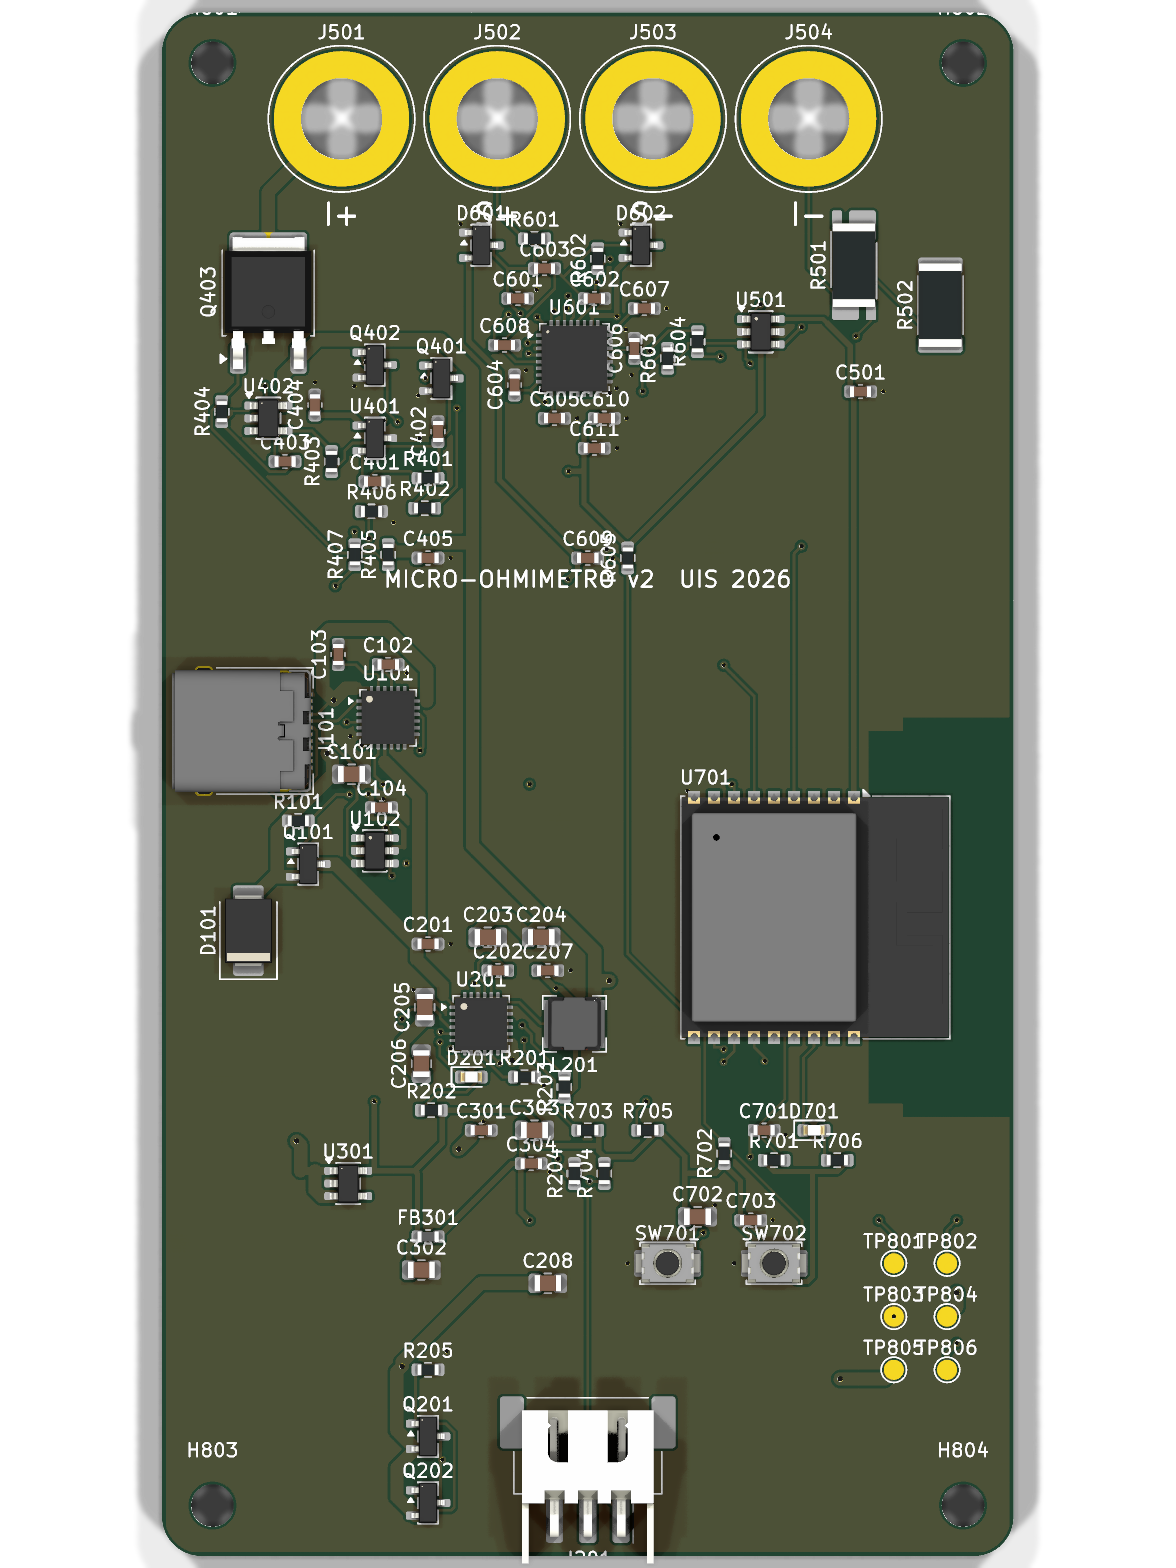
\includegraphics[width=\textwidth]{pcb_3d_superior.png}\caption{Superior}\end{subfigure}
\begin{subfigure}{0.32\textwidth}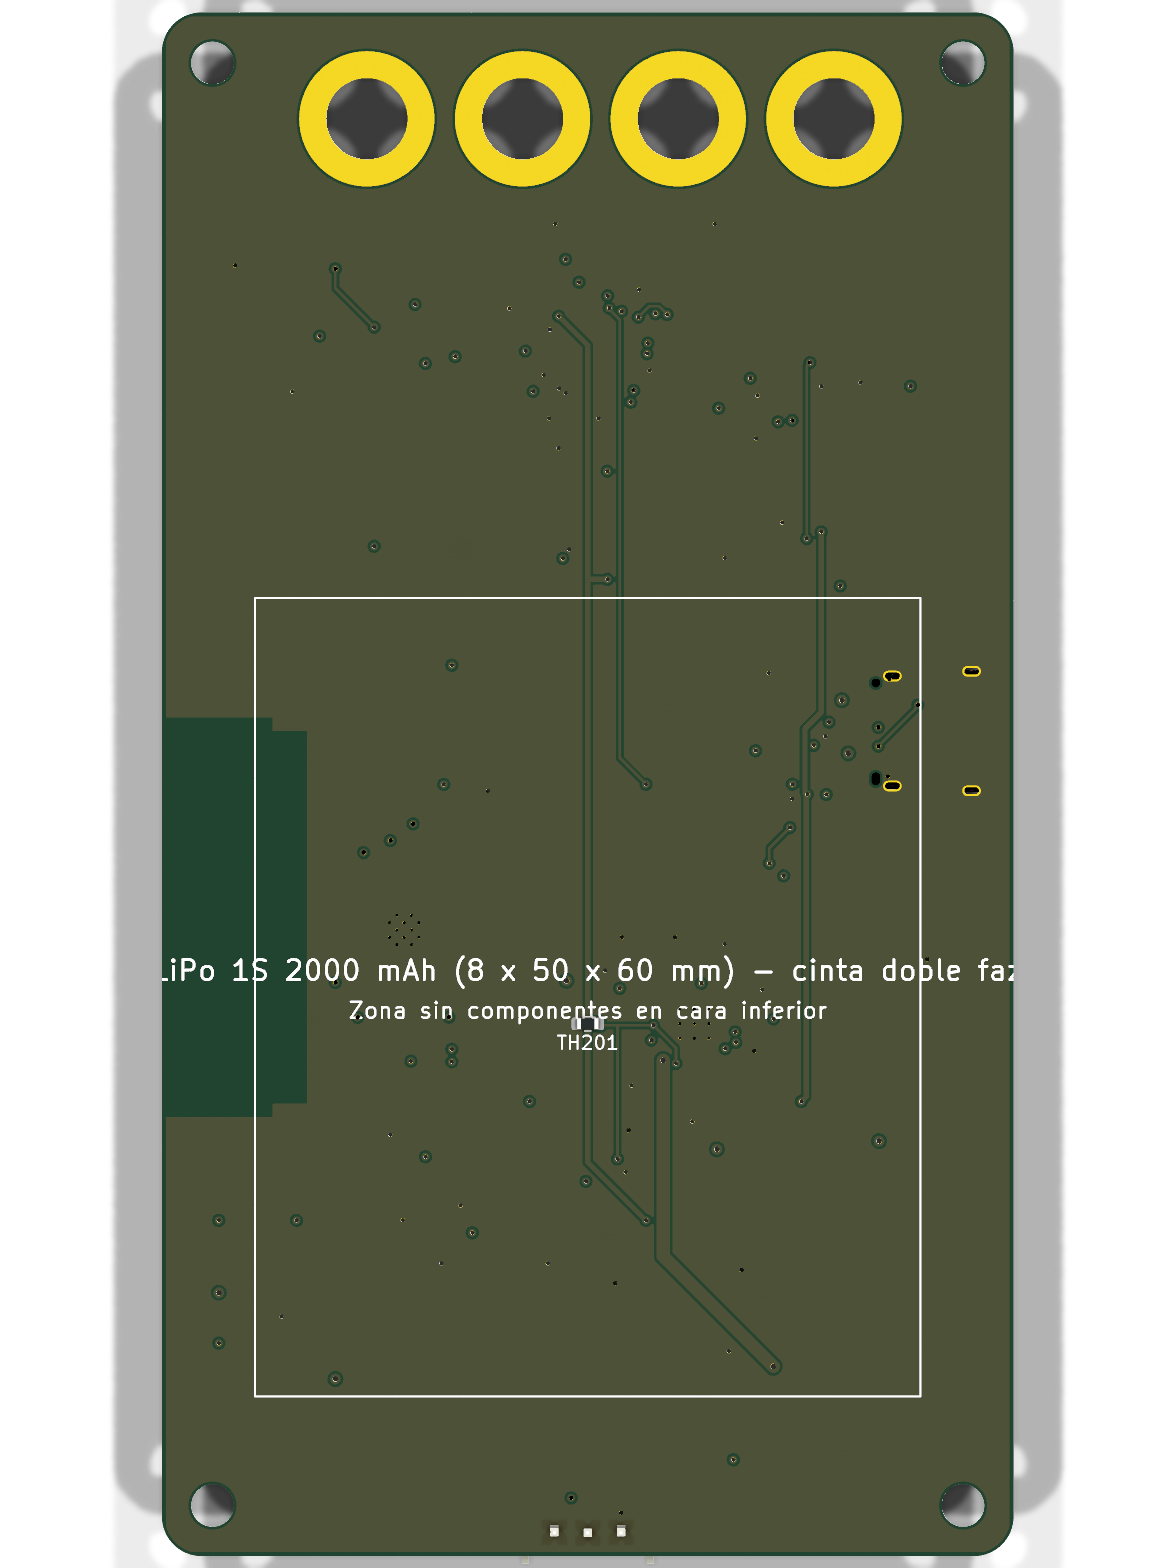
\includegraphics[width=\textwidth]{pcb_3d_inferior.png}\caption{Inferior (silueta de la LiPo)}\end{subfigure}
\begin{subfigure}{0.32\textwidth}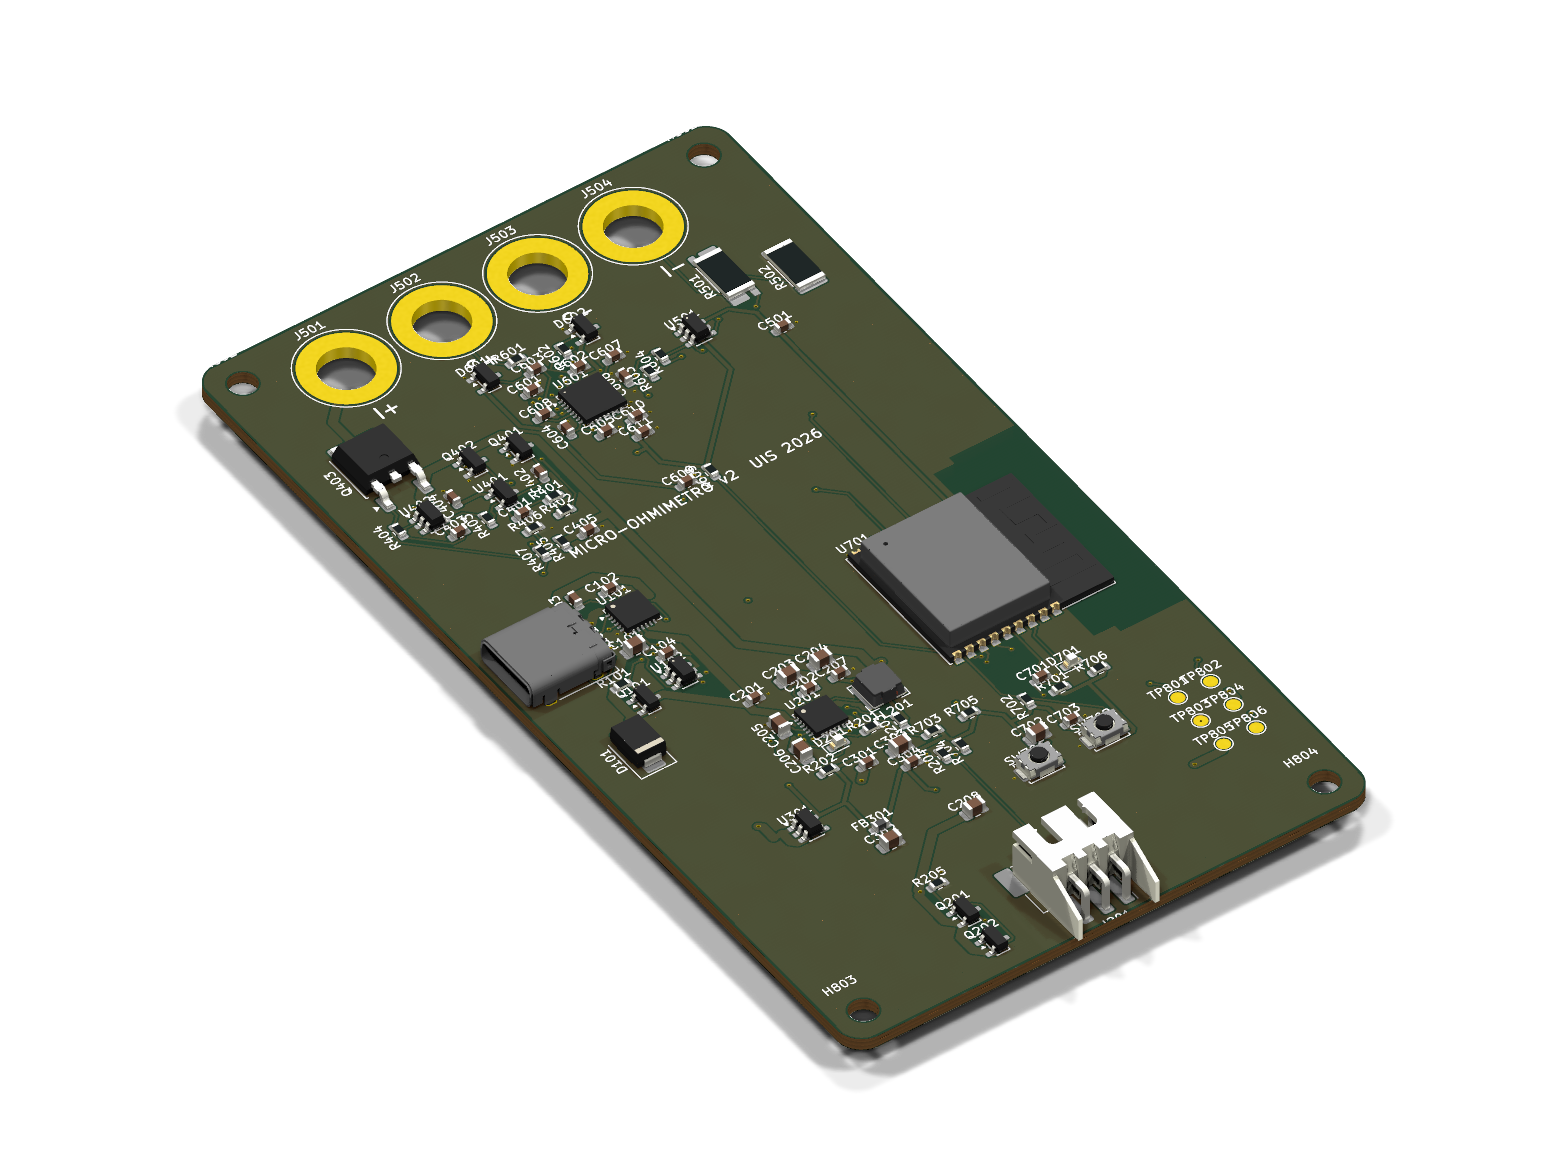
\includegraphics[width=\textwidth]{pcb_3d_iso.png}\caption{Isométrica}\end{subfigure}
\caption{Vistas 3D de la PCB (render de KiCad 10).}\label{fig:pcb3d}
\fuente{\repof{hardware/kicad/microohmetro_v2.kicad_pcb}; modelo STEP en \repof{hardware/fabricacion/microohmetro_v2.step}.}
\end{figure}

\begin{figure}[H]\centering
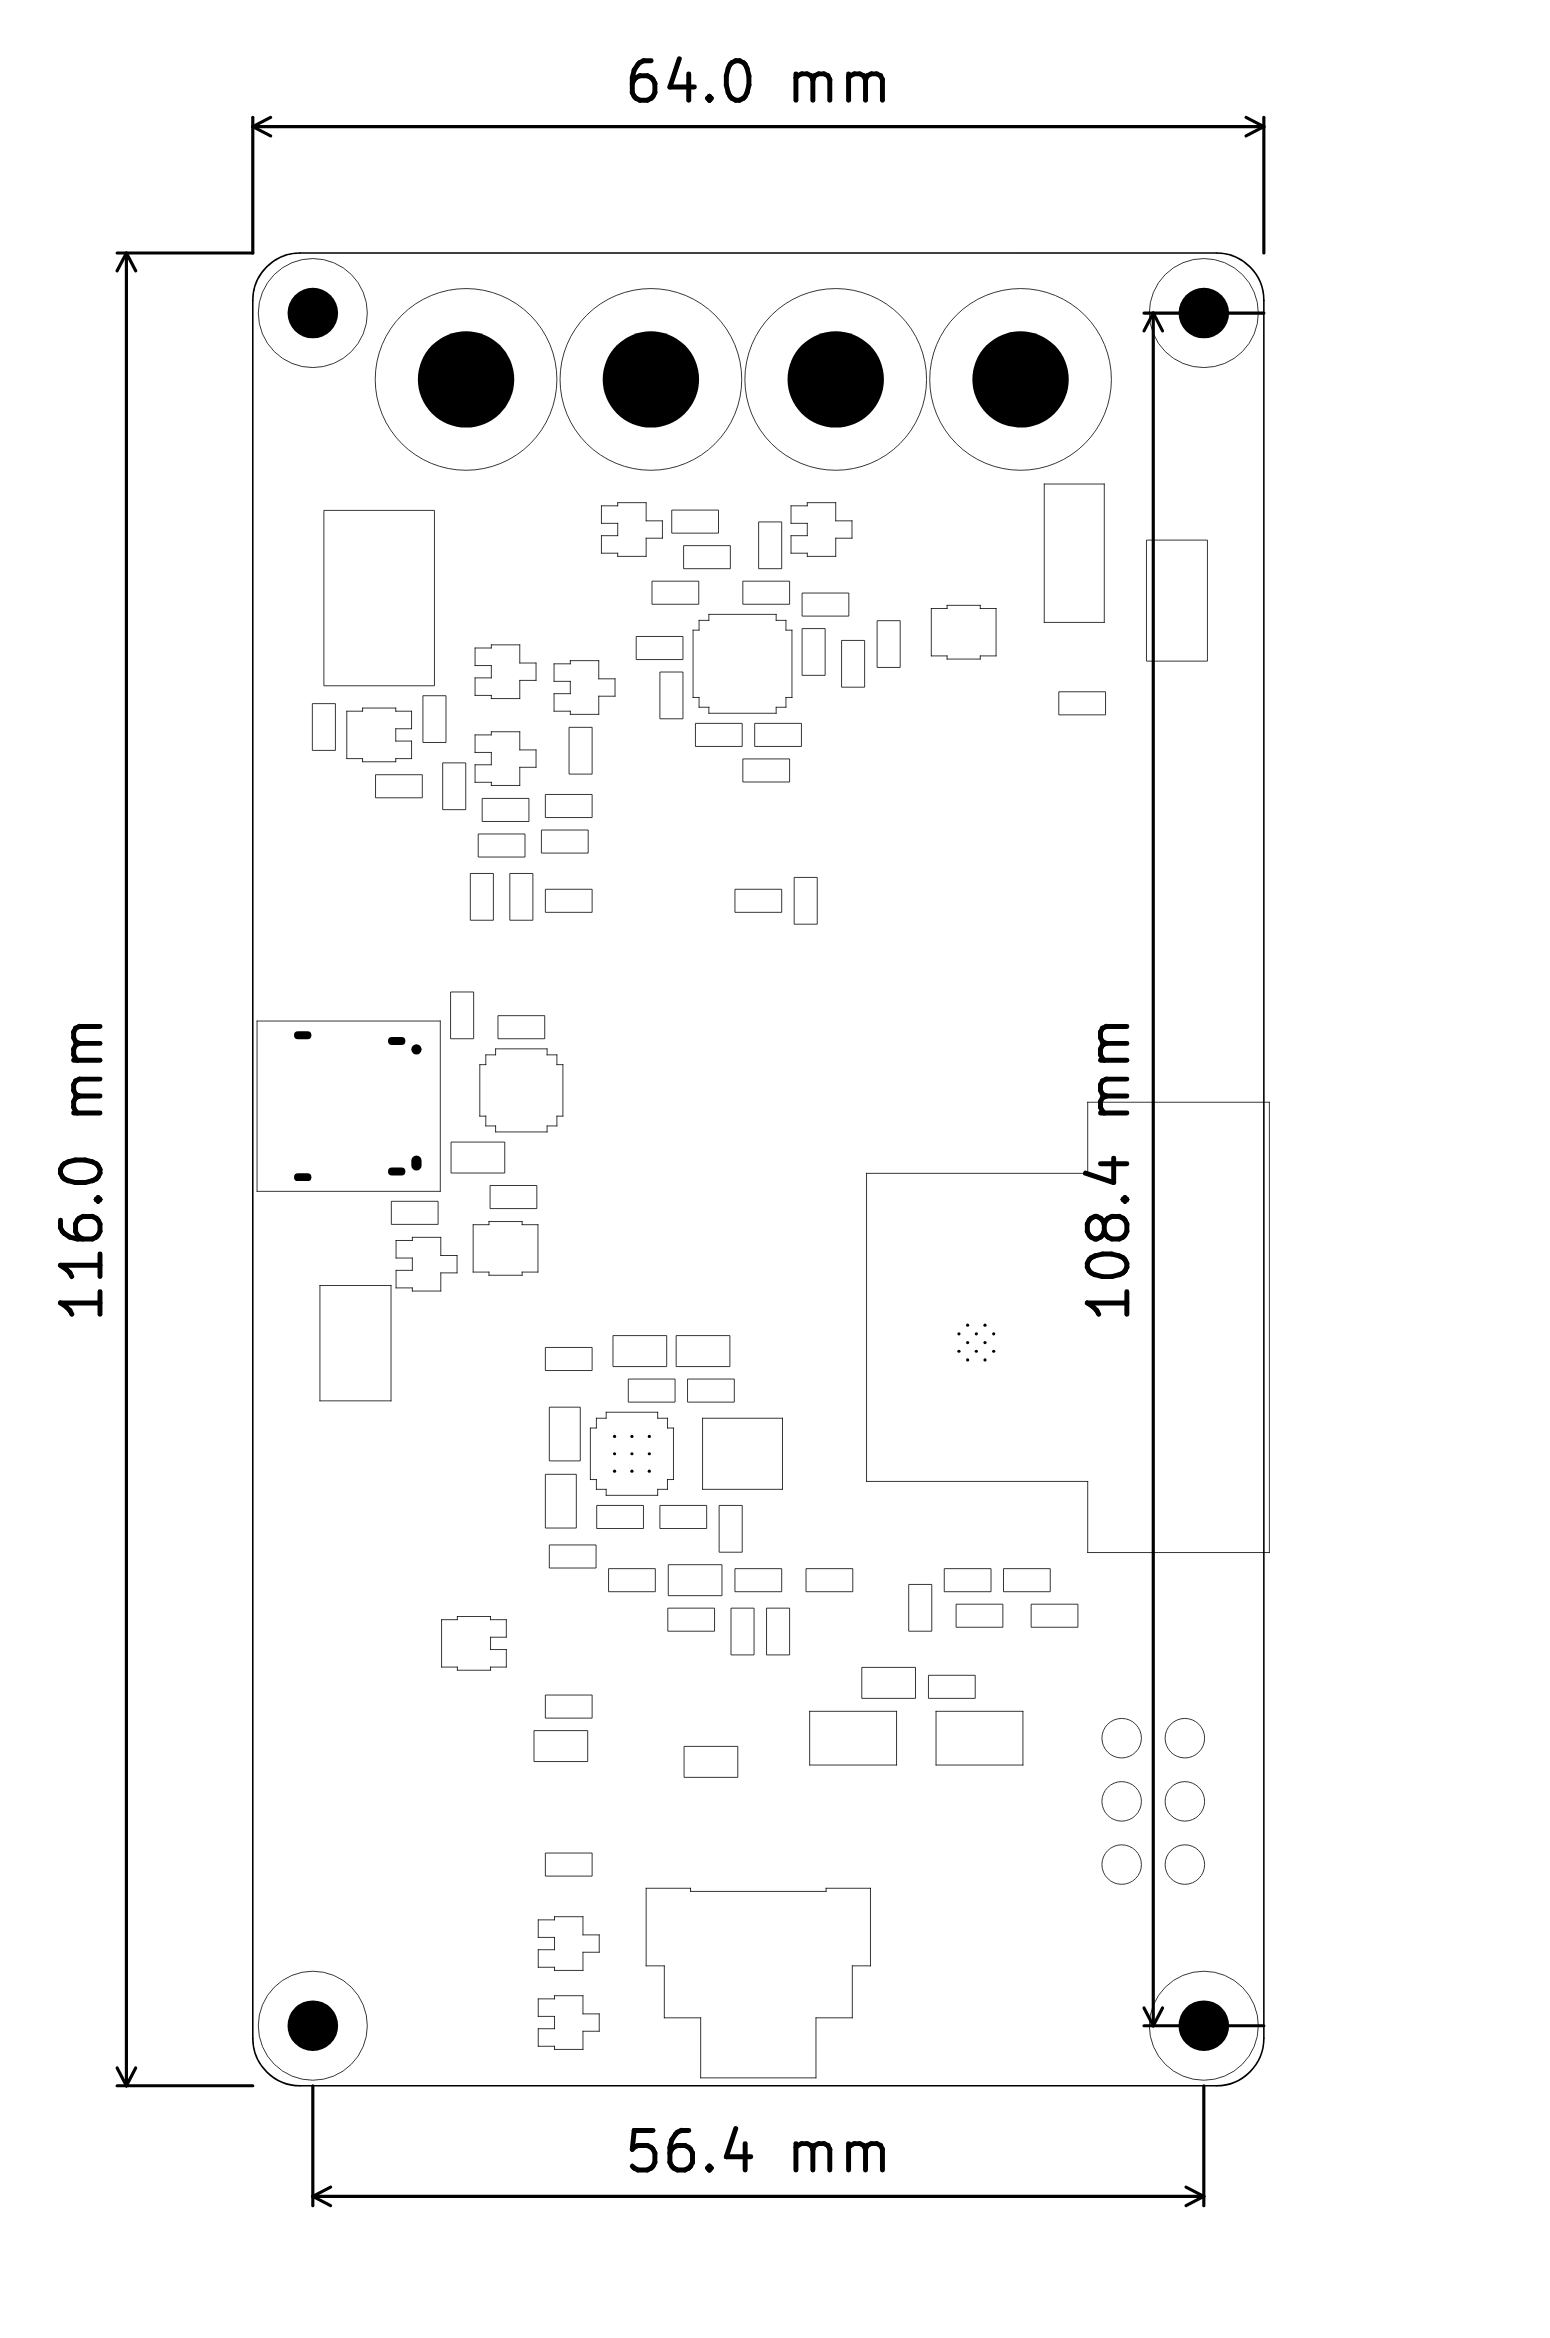
\includegraphics[height=0.62\textheight]{pcb_plano_acotado.png}
\caption{Plano mecánico acotado: 64\,mm $\times$ 116\,mm.}\label{fig:plano}\end{figure}

\begin{table}[H]\centering\small
\caption{Especificaciones físicas de la PCB.}\label{tab:pcbspec}
\begin{tabular}{ll}\toprule
Dimensiones & 64\,mm $\times$ 116\,mm (esquinas R = 3 mm), 4 agujeros M3\\
Capas / espesor / cobre & 4 / 1,6 mm / 1 oz\\
Pista / holgura mínima & 0,15 mm / 0,15 mm\\
Vía estándar / mínima & 0,6/0,3 mm; vías térmicas de 0,2 mm\\
Acabado sugerido & ENIG (pads finos LFCSP/QFN)\\
Montaje & SMD (excepto bornes banana), cara superior\\\bottomrule
\end{tabular}\end{table}

\textbf{Estado}: el DRC no reporta cortocircuitos ni violaciones de holgura; quedan unas 7 conexiones cortas por completar manualmente en KiCad (VBUS\_C, +3V3, SYS, PMID, I2C\_SDA) y advertencias de serigrafía. \PENDIENTE{cerrar esas conexiones y repetir el DRC antes de fabricar.}

% =====================================================================================
\section{Materiales, BOM y datasheets}
\begin{table}[H]\centering\small
\caption{Materiales de resistencias y capacitores.}\label{tab:materiales}
\begin{tabularx}{\textwidth}{lY}\toprule
$R_S$ (0,12 $\Omega$) & Shunt de 4 terminales en metal strip 2512, 1 W, TCR $\leq$ 50 ppm/°C, 0,1 \% recomendado\\
Ganancia/referencia/filtro & Thin film 0,1 \%, $\leq$ 25 ppm/°C\\
Resto de resistencias & Thick film 0603, 1 \%\\
Ruta de señal & MLCC C0G/NP0 (sin efecto piezoeléctrico ni de \emph{DC bias})\\
Desacoplo y bulk & MLCC X7R con tensión nominal $\geq$ 2$\times$ la de trabajo\\\bottomrule
\end{tabularx}\end{table}

\begin{table}[H]\centering\small
\caption{Componentes principales y enlaces a datasheets.}\label{tab:ds}
\begin{tabular}{lll}\toprule
Ref. & Componente & Datasheet\\\midrule
U601 & AD7124-4BBCPZ-RL7 & \href{https://www.analog.com/media/en/technical-documentation/data-sheets/ad7124-4.pdf}{analog.com}\\
U401 & REF3325AIDBZR & \href{https://www.ti.com/lit/ds/symlink/ref3325.pdf}{ti.com}\\
U402 & OPA388IDBVR & \href{https://www.ti.com/lit/ds/symlink/opa388.pdf}{ti.com}\\
U501 & INA181A1IDBVR & \href{https://www.ti.com/lit/ds/symlink/ina181.pdf}{ti.com}\\
Q403 & NTD25P03LT4G & \href{https://www.onsemi.com/pdf/datasheet/ntd25p03l-d.pdf}{onsemi.com}\\
R501 & WSK2512 (0,12 $\Omega$) & \href{https://www.vishay.com/docs/30108/wsk2512.pdf}{vishay.com}\\
U201 & BQ25895RTWR & \href{https://www.ti.com/lit/ds/symlink/bq25895.pdf}{ti.com}\\
U101 & STUSB4500QTR & \href{https://www.st.com/resource/en/datasheet/stusb4500.pdf}{st.com}\\
U301 & AP2112K-3.3 & \href{https://www.diodes.com/assets/Datasheets/AP2112.pdf}{diodes.com}\\
U701 & ESP32-C3-WROOM-02-N4 & \href{https://www.espressif.com/sites/default/files/documentation/esp32-c3-wroom-02_datasheet_en.pdf}{espressif.com}\\
U102 & USBLC6-2SC6 & \href{https://www.st.com/resource/en/datasheet/usblc6-2.pdf}{st.com}\\
Q101, Q201/202 & AO3401A & \href{https://www.aosmd.com/res/datasheets/AO3401A.pdf}{aosmd.com}\\\bottomrule
\end{tabular}\end{table}
La BOM completa (103 componentes, con MPN, footprint y especificación) está en \repof{docs/bom_kicad.csv}.

% =====================================================================================
\section{Aplicación móvil}
La aplicación Android (Flutter) se conecta por BLE, muestra la resistencia en m$\Omega$, el estado de la batería y de la carga, la gráfica temporal y el historial, e incluye un simulador. En la versión 2 los rangos de la aplicación corresponden a los tres rangos automáticos del PGA.
\begin{figure}[H]\centering
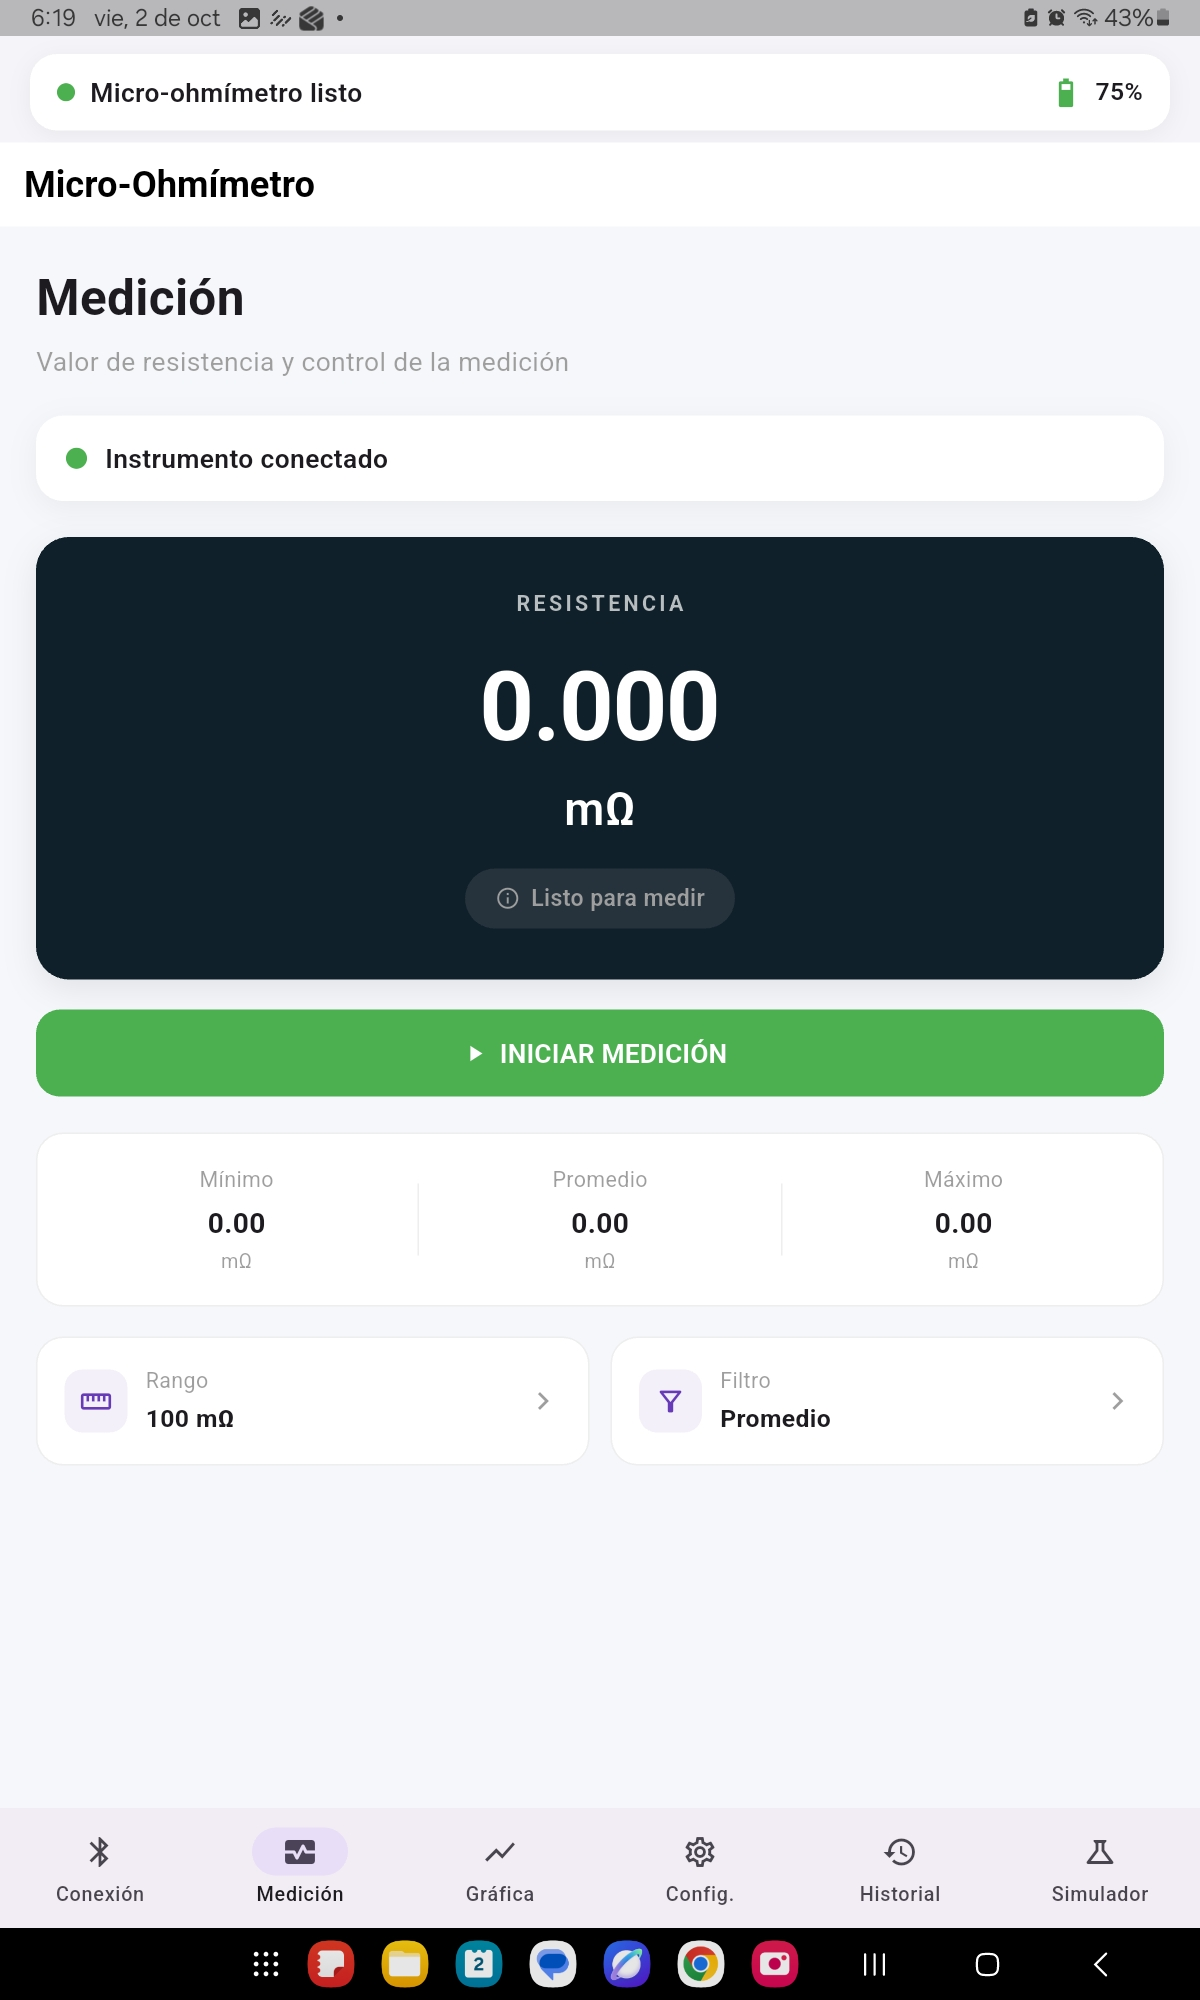
\includegraphics[height=6cm]{MEDICION.jpeg}\hspace{6mm}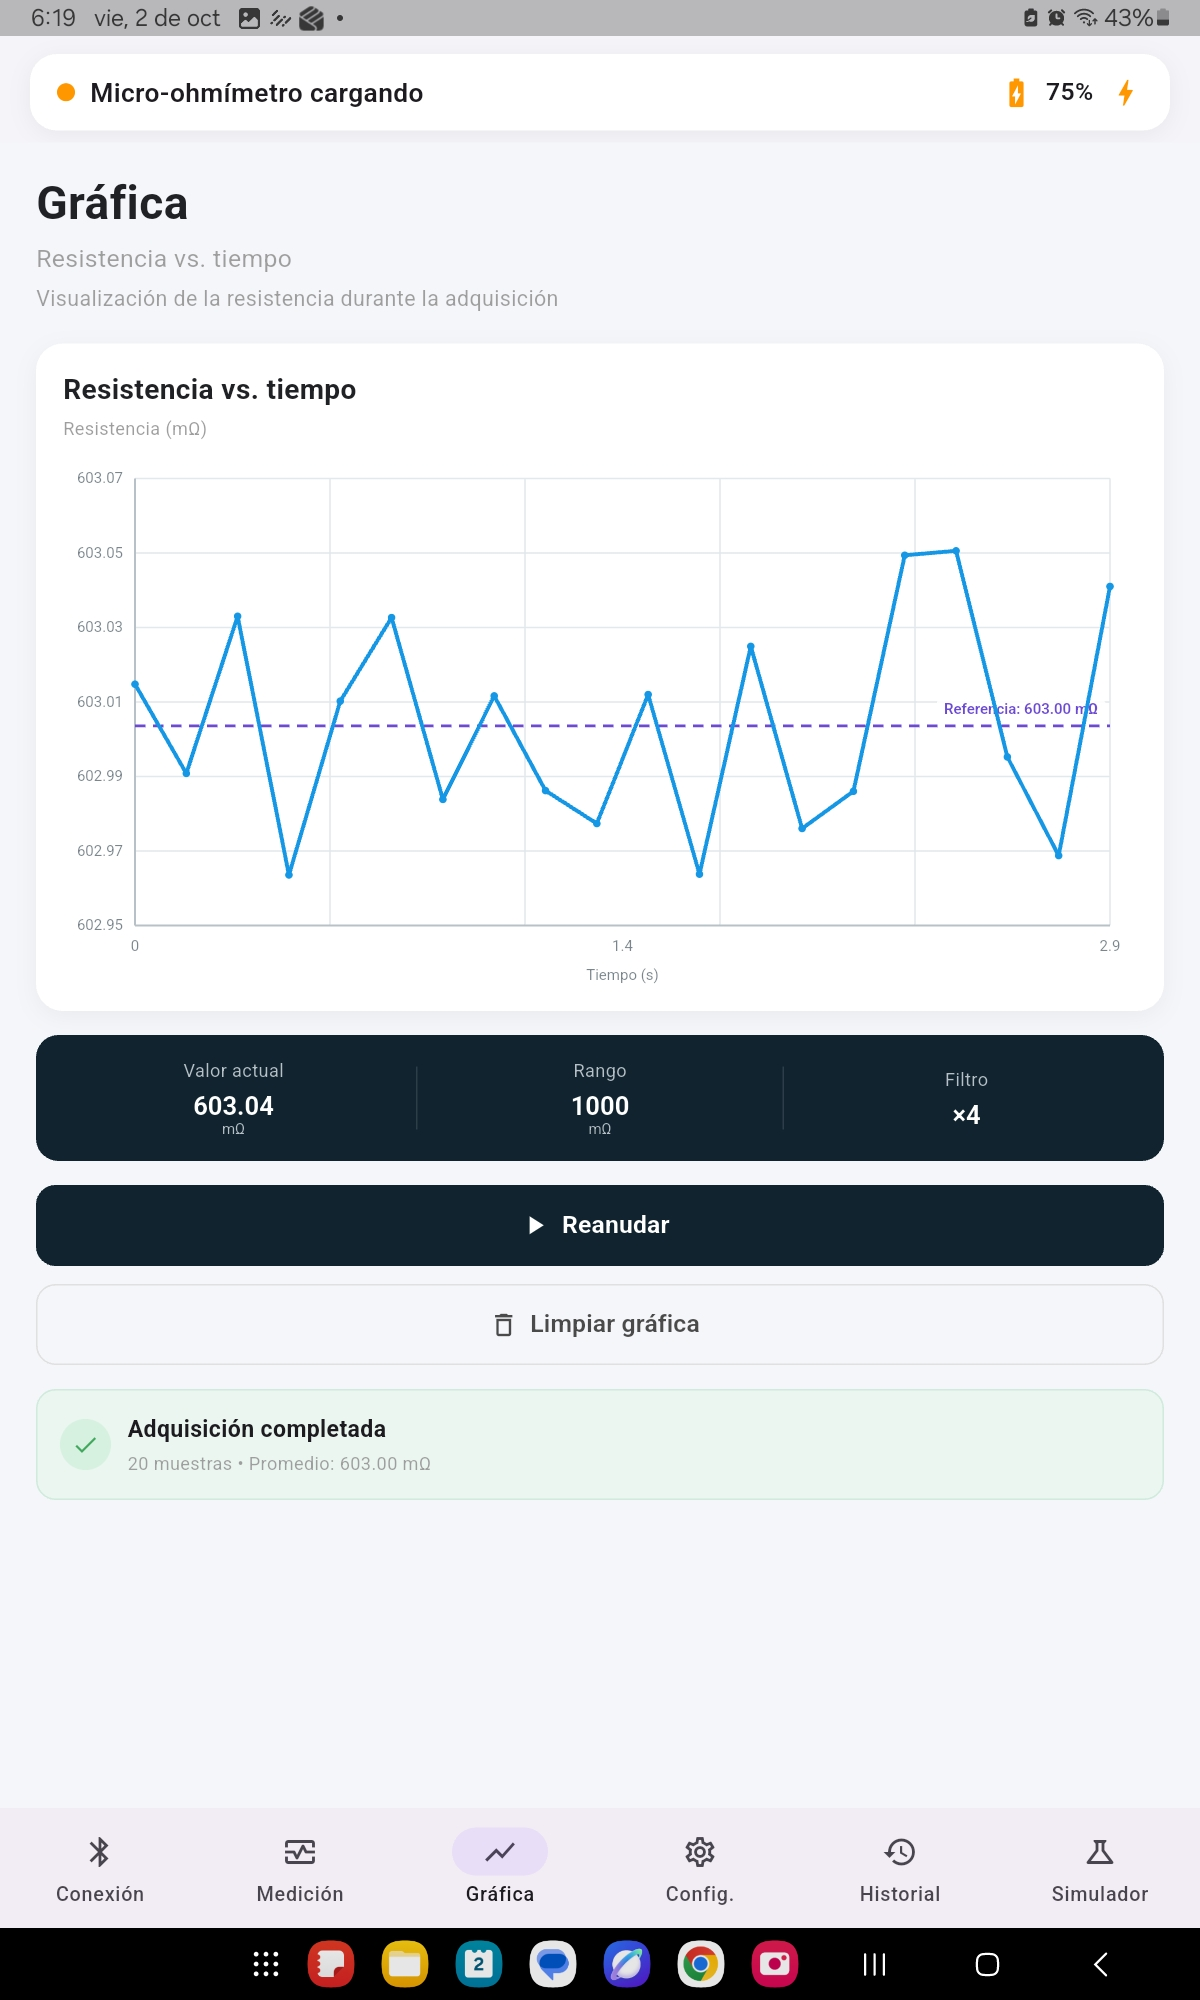
\includegraphics[height=6cm]{GRAFICA.jpeg}
\caption{Pantallas de medición y gráfica de la aplicación.}\label{fig:app}\end{figure}

% =====================================================================================
\section{Conclusiones}
\begin{enumerate}[nosep]
\item La corriente pulsada de \SI{1,04}{A} multiplica por 10 la señal (\SI{1}{mV} en \SI{1}{m\ohm}) y mantiene la disipación media del P-MOS en \SI{0,43}{W}.
\item La medición ratiométrica de dos niveles elimina la dependencia de la referencia, de la ganancia del INA y del valor de la corriente, y cancela offsets y FEM termoeléctricas (S3: $\pm$\SI{0,96}{\percent} $\to$ \SI{0}{\percent}).
\item Usar el PGA del AD7124 en lugar del amplificador diferencial discreto reduce la dispersión de \SI{88}{\percent} a \SI{0,057}{\percent} ($\sigma$, Montecarlo).
\item El único componente crítico por tolerancia es el shunt: se recomienda uno de 0,1 \% o una calibración única contra un patrón.
\item El sistema de energía (PD 9 V, carga de 2 A, polaridad inversa) permite cargar en $\approx$1,5 h y medir $\approx$10 h.
\end{enumerate}

\section{Trabajo futuro}
Completar las conexiones pendientes de la PCB y el DRC; fabricar y caracterizar con resistencias patrón (\SI{1}{m\ohm}--\SI{1}{\ohm}); medir el consumo real del ESP32-C3; validar la estabilidad térmica del shunt y del P-MOS; cerrar el protocolo BLE con la aplicación.

% =====================================================================================
\appendix
\section{Esquemático completo (hojas de detalle)}\label{anx:sch}
\begin{figure}[H]\centering\includegraphics[page=2,width=\textwidth]{esquematico_v2.pdf}\caption{Esquemático, página 2: Entrada USB-C y Power Delivery.}\end{figure}
\begin{figure}[H]\centering\includegraphics[page=3,width=\textwidth]{esquematico_v2.pdf}\caption{Esquemático, página 3: Cargador y batería.}\end{figure}
\begin{figure}[H]\centering\includegraphics[page=4,width=\textwidth]{esquematico_v2.pdf}\caption{Esquemático, página 4: Regulación 3,3 V.}\end{figure}
\begin{figure}[H]\centering\includegraphics[page=8,width=\textwidth]{esquematico_v2.pdf}\caption{Esquemático, página 8: Microcontrolador ESP32-C3.}\end{figure}
\begin{figure}[H]\centering\includegraphics[page=9,width=\textwidth]{esquematico_v2.pdf}\caption{Esquemático, página 9: Mecánicos y puntos de prueba.}\end{figure}


\section{Repositorio de respaldo}
\begin{itemize}[nosep]
\item Hardware (KiCad, librerías, 3D, Gerbers): \href{\repo/tree/v1.0/hardware}{\texttt{github.com/.../tree/v1.0/hardware}}
\item Simulaciones PSpice (\texttt{.cir}, modelos y datos \texttt{.csv}): \href{\repo/tree/v1.0/simulaciones}{\texttt{github.com/.../tree/v1.0/simulaciones}}
\item Imágenes en alta resolución: \href{\repo/tree/v1.0/imagenes}{\texttt{github.com/.../tree/v1.0/imagenes}}
\item Documentos de diseño, informes por etapa y BOM: \href{\repo/tree/v1.0/docs}{\texttt{github.com/.../tree/v1.0/docs}}
\end{itemize}
\end{document}
